% LTeX: language=de_DE
\documentclass{uebung_cs}
\usepackage{algo223}
\uebung{5}{}{}
\blattname{Übungen zu Woche 5: Randomisierte Algorithmen I}

%%%%%%%%%%%%%%%%%%%%%%%%%%%%%%%%%%%%%%%%%%%%%%%%%%%%%%%%%%%%%%%%%%%%%%%%%%%%
\begin{document}

\section*{Dienstag}

\begin{exercise}[Contention Resolution][\athome\easy]\
	% Algorithms and Data Structures 2 - randomizedI.pdf
	Führe das \textit{contention resolution} Protokoll mit $4$ Prozessen von Hand aus. Benutze hierzu zwei Münzen und werfe sie, um die zufällige Auswahl zu simulieren.
	Wie viele Runden hast du gebraucht, bis alle Prozesse erfolgreich auf die Datenbank zugegriffen haben?
	Inwiefern passt dein Ergebnis zu der theoretisch vorhergesagten Anzahl an benötigten Runden zusammen?
\end{exercise}    

\begin{exercise}[Mehrheit][\href{https://moodle.studiumdigitale.uni-frankfurt.de/moodle/mod/assign/view.php?id=239323}{moodle}\athome]
	% Algorithms and Data Structures 2 - randomizedI.pdf
	Gegeben ist eine Sequenz $x_1,x_2,\dots,x_n$ von $n$ ganzen Zahlen. Die Sequenz hat das \textit{Mehrheitselement}~$t$, wenn die Zahl $t$ öfter als $\frac{n}{2}$-mal in der Sequenz vorkommt. Zum Beispiel hat die Sequenz $1,2,3,1,2,2,2$ das Mehrheitselement $2$, während die Sequenz $2,2,1,2,3,3$ kein Mehrheitselement hat. Im Folgenden ist der randomisierte Algorithmus \textsc{FindeMehrheitsElement} beschrieben, der das Mehrheitselement finden soll.
	
	\begin{quote}
		\textsc{FindeMehrheitsElement}$(x_1,\dots,x_n)$: \\
		Ziehe einen Index $i$ uniform zufällig aus $\{1,\dots,n\}$. Prüfe dann, ob $x_i$ öfter als $\frac{n}{2}$-mal in der Sequenz vorkommt. Wenn ja, dann gib $x_i$ aus. Ansonsten gib aus, dass es kein Mehrheitselement gibt.
	\end{quote}
	\begin{enumerate}
		\item\easy Was ist die Laufzeit von \textsc{FindeMehrheitsElement}?
		\item\easy Kann \textsc{FindeMehrheitsElement} ein Mehrheitselement zurückgeben, wenn die Sequenz keines hat? Begründe deine Antwort.
		\item\easy Kann \textsc{FindeMehrheitsElement} ausgeben, dass kein Mehrheitselement existiert, obwohl die Sequenz ein solches besitzt? Begründe deine Antwort.
		\item\medium Bestimme die Wahrscheinlichkeit, dass \textsc{FindeMehrheitsElement} eine falsche Antwort liefert.
	\end{enumerate}
\end{exercise}

\begin{exercise}[Wahrscheinlichkeitsrechnung][\atschool]\
	% Algorithms and Data Structures 2 - randomizedI.pdf
	\begin{enumerate}
		\item\easy
		Seien $E$ und $F$ zwei Ereignisse mit $\Pr(E | F) = \Pr(E)$ und $\Pr(F | E) = P(F)$. Zeige, dass dann auch $\Pr(E \cap F) = \Pr(E) \cdot \Pr(F)$ gilt.
		\tipp{Benutze die Definition der bedingten Wahrscheinlichkeit}
		\item\medium
		Betrachte die folgende Anwendung der \textit{union bound} auf den Folien zu \textit{contention resolution} mit $n$ Prozessen:
		\[
			\Pr\left(\bigcup_{i=1}^n F_{i,t}\right)
			\le
			\sum_{i=1}^n \Pr(F_{i,t})\,.
		\]
		Hierbei ist $F_{i,t}$ das Ereignis, dass Prozess $i$ es in keiner der Runden $1,\dots,t$ geschafft hat, auf die Datenbank zuzugreifen.
		Sind die einzelnen Ereignisse~$F_{i,t}$ hierbei disjunkt oder überschneiden sie sich? Warum?
	\end{enumerate}
\end{exercise}

\section*{Donnerstag}

\begin{exercise}[Minimaler Schnitt][\athome]
	% Algorithms and Data Structures 2 - randomizedI.pdf
	Betrachte den Beispielgraphen zum Kontraktionsalgorithmus aus der Vorlesung:
	\begin{center}
	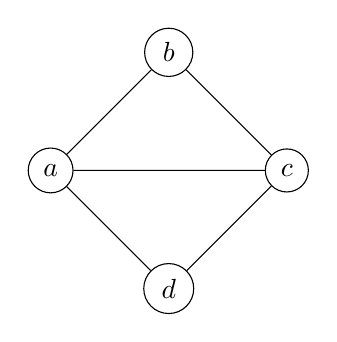
\begin{tikzpicture}
            \node[draw,circle] (a) at (0,0) {$a$};
            \node[draw,circle] (b) at (1.5,1.5) {$b$};
            \node[draw,circle] (d) at (1.5,-1.5) {$d$};
            \node[draw,circle] (c) at (3,0) {$c$};
            
            \draw  (a) -- (b)
                   (a) -- (c)
                   (a) -- (d)
                   (b) -- (c)
                   (c) -- (d);
        \end{tikzpicture}
	\end{center}
	\begin{enumerate}
		\item\easy Zeige, dass es eine Sequenz von Kontraktionen gibt, die zu einem nicht-minimalen Schnitt führt.
		\item\medium Berechne die genaue Wahrscheinlichkeit dafür, dass der Kontraktionsalgorithmus den minimalen Schnitt ausgibt.
	\end{enumerate}
\end{exercise}

\begin{exercise}[Schneller Kontraktionsalgorithmus][\href{https://moodle.studiumdigitale.uni-frankfurt.de/moodle/mod/assign/view.php?id=239326}{moodle}\athome\\\medium]
	% Algorithms and Data Structures 2 - randomizedI.pdf
	Wie kann man den Kontraktionsalgorithmus für minimale Schnitte effizient implementieren? Beschreibe deine Lösung als Pseudocode, unter Verwendung aller nötigen Datenstrukturen und Algorithmen. Analysiere die Laufzeit sowie den Platzverbrauch.
\end{exercise}

\begin{exercise}[Kontraktionsalgorithmus analysieren][\atschool]
	% Algorithms and Data Structures 2 - randomizedI.pdf
	Wir vervollständigen jetzt die Analyse der Erfolgswahrscheinlichkeit des Kontraktionsalgorithmus. Die folgende Herleitung führt zum gewünschten Ergebnis:
	\begin{align}
		&\nonumber\Pr(E_{n-2} \cap \cdots \cap E_1) \\
		&= \Pr(E_{n-3} \cap \cdots \cap E_1) \cdot \Pr(E_{n-2}|E_{n-3} \cap \cdots \cap E_1) \\
		&= \Pr(E_1) \cdot \Pr(E_2|E_1) \cdots \Pr(E_{j+1} | E_j \cap \cdots \cap E_1) \cdots \Pr(E_{n-2} | E_{n-3} \cap \cdots \cap E_1) \\
		&\ge \left(1 - \frac{2}{n} \right) \cdot \left(1 - \frac{2}{n-1} \right) \cdot \left(1 - \frac{2}{n-2} \right) \cdots \left(1 - \frac{2}{3} \right) \\
		&= \left(\frac{n-2}{n}\right) \cdot \left(\frac{n-3}{n-1}\right) \cdot \left(\frac{n-4}{n-2}\right) \cdots \left(\frac{2}{4}\right) \cdot \left(\frac{1}{3}\right) \\
		&= \left(\frac{2}{n(n-1)}\right) \geq \frac{2}{n^2}
	\end{align}
	\begin{enumerate}
		\item\easy\label{conditional} Zeige~(1) formal, indem du die Definition der bedingten Wahrscheinlichkeit benutzt. Erkläre außerdem die Intuition, indem du dir bewusst machst, was die linke und rechte Seite bedeuten.
		\item\mittel Zeige (2). \tipp{Wende die Aussage aus Teilaufgabe~\ref{conditional} induktiv an}
		\item\easy Zeige (3), indem du jeden Faktor einzeln abschätzt.
		\item\mittel Zeige (4). \tipp{Teleskopprodukt}
		\item\easy Zeige (5) durch elementare Algebra.
	\end{enumerate}
\end{exercise}

\clearpage
\section*{Weitere Aufgaben und Projekte}

\begin{exercise}[Zufällige Konfliktfreiheit][\projekt]
	In Abschnitt 13.1 (\textbf{KT}) haben wir ein einfaches verteiltes Protokoll gesehen, um ein \textit{contention resolution} Problem zu lösen. Eine zweite Möglichkeit, um \textit{contention resolution} mittels Randomisierung zu lösen, ist eine verteilte Konstruktion eines Independent Set.

	In einem System mit $n$ Aufgaben $P_1,\dots,P_n$ stehen einige Paare von Aufgaben miteinander im Konflikt, beispielsweise wenn beide Aufgaben Zugang zu derselben Ressource brauchen. Das Ziel ist es, in einem gegebenen Zeitintervall eine möglichst große Menge~$S$ von ausführbaren Aufgaben zu finden, sodass keine zwei Aufgaben aus $S$ in einem Konflikt stehen. Die Menge~$S$ nennen wir \textit{konfliktfrei}.
	
	Diesen Vorgang kann man sich als einen Graphen $G = (V,E)$ vorstellen. Dabei repräsentiert jeder Knoten $v \in V$ eine Aufgabe und eine Kante $e = (u,v)$ stellt einen Konflikt zwischen zwei Aufgaben $u$ und $v$ dar. Ist eine Menge~$S$ von Aufgaben konfliktfrei, bilden sie eine \emph{unabhängige Menge} (\emph{independent set}) in $G$. 
	Es ist im Allgemeinen schwierig, eine maximale und konfliktfreie Menge~$S$ für einen beliebigen Konfliktgraphen~$G$ zu finden.
	
	Deshalb benutzen wir eine Heuristik mit einer einfachen dezentralisierten Methode, die eine vernünftig große und konfliktfreie Menge findet: Jede Aufgabe \enquote{kommuniziert} nur mit den Aufgaben, mit denen sie in Konflikt steht, und entscheidet dann, ob sie in die Menge~$S$ gehört oder nicht.
	Wir nehmen an, dass der Konfliktgraph~$G$ $d$-regulär ist, das heißt, jeder Knoten hat genau~$d$ Nachbarn. Schaue dir nun das folgende Verfahren an:
	
	\begin{quote}
		\textsc{FindeKonfliktfreieMenge}: \\
		Jede Aufgabe $P_i$ wählt unabhängig einen zufälligen Wert $x_i$. Dabei nimmt $x_i$ mit einer Wahrscheinlichkeit von $\frac{1}{2}$ den Wert $0$ und mit einer Wahrscheinlichkeit von $\frac{1}{2}$ den Wert $1$ an. Die Aufgabe kommt genau dann in die Menge $S$, wenn sie $x_i = 1$ gewählt hat und jede Aufgabe, mit der sie im Konflikt steht, den Wert $0$ gewählt hat.
	\end{quote}
	
		\begin{enumerate}
		\item\medium Beweise, dass die durch \textsc{FindeKonfliktfreieMenge} entstehende Menge~$S$ immer konfliktfrei ist.
		\item\hard Gib außerdem eine Formel für $\mathbf{E}[|S|]$ an, also die erwartete Größe von $S$, in Abhängigkeit von der Anzahl $n$ an Aufgaben und der Anzahl~$d$ an Konflikten pro Aufgabe. Begründe, warum deine Formel korrekt ist.
	\end{enumerate}
\end{exercise}

\end{document}
